% Informe final — Proyecto de Visión Computacional (UCB)
% Compilar: tectonic main.tex   (o subir informe/ a Overleaf / pdfLaTeX)
\documentclass[11pt,a4paper]{article}

\usepackage[utf8]{inputenc}
\usepackage[T1]{fontenc}
\usepackage[spanish,es-noshorthands]{babel}
\usepackage[margin=2.3cm]{geometry}
\usepackage{graphicx}
\usepackage{booktabs}
\usepackage{float}
\usepackage{amsmath}
\usepackage{caption}
\usepackage{enumitem}
\usepackage{xcolor}
\usepackage{tabularx}
\usepackage{array}
\usepackage{microtype}
\usepackage[hidelinks]{hyperref}

\captionsetup{font=small,labelfont={bf}}
\setlength{\parskip}{0.4em}
\setlength{\parindent}{0pt}

\title{}
\author{}
\date{}

\begin{document}

% ============================ 1. PORTADA ============================
\begin{titlepage}
  \centering
  
\includegraphics[width=0.32\textwidth]{figures/ucb-logo.png}\\[1.0em]
  {\Large\bfseries Universidad Católica Boliviana ``San Pablo''}\\[0.4em]
  {\large Maestría en Ciencia de Datos e Inteligencia Artificial Aplicada\\[0.2em]
  Módulo: Visión Computacional}\\[1.8em]
  \rule{\textwidth}{0.6pt}\\[1.0em]
  {\LARGE\bfseries Detección y clasificación de defectos en superficies
  metálicas con aprendizaje profundo: del entrenamiento en GPU a una demo
  web en tiempo real}\\[0.8em]
  \rule{\textwidth}{0.6pt}\\[1.8em]
  {\large\bfseries Equipo de Proyecto}\\[0.8em]
  \begin{tabular}{ll}
    \textbf{Simon Alex Rodriguez Saavedra} & \emph{Líder / Integrador} \\
    \textbf{Jennifer Suarez Gutierrez} & \emph{Entrenamiento CNN baseline} \\
    \textbf{Daniel Ribera Añez} & \emph{Contribuidor} \\
    \textbf{Daniela Alejandra Caro Arrazola} & \emph{Contribuidora} \\
  \end{tabular}\\[2.0em]
  {\large Agosto 2026}\\[0.5em]
  \vfill
  \begin{minipage}{0.95\textwidth}
    \small\centering
    \textbf{Repositorio del proyecto (código fuente, datos, modelos y demo web):}\\
    \url{https://github.com/SimonLexRS/vision-computacional}
  \end{minipage}
\end{titlepage}

% ============================ 2. RESUMEN ============================
\section*{Resumen}
\addcontentsline{toc}{section}{Resumen}

Este proyecto presenta el desarrollo, evaluación y despliegue de un sistema de
inspección automatizada para la detección y clasificación de defectos superficiales
en piezas metálicas, optimizado para entornos de acero laminado. Frente a la
variabilidad, subjetividad y fatiga asociadas al control de calidad manual, se
propone una arquitectura jerárquica de dos etapas orientada al balance óptimo entre
eficiencia computacional y precisión analítica: (1) un clasificador de dominio
(\emph{Gate}) basado en MobileNetV3-Small (1.5M parámetros) que actúa como filtro
binario de alta velocidad para discriminar si la escena es una superficie metálica
válida o descartar entradas fuera de dominio (OOD), seguido de (2) un detector
YOLOv8n (3.2M parámetros) para la localización multiclase y acotación mediante cajas
delimitadoras de las fallas detectadas.

El entrenamiento se realizó sobre un dataset híbrido de 17\,250 imágenes combinando
muestras sintéticas con benchmarks reales de la industria (\emph{SteelDefectX} y
\emph{NEU-DET}). Los resultados cuantitativos evidencian un desempeño sobresaliente,
alcanzando un F1-Macro de $1.0000$ en la clasificación de dominio y un $\text{mAP}_{50}$
de $0.739$ ($\text{mAP}_{50\text{--}95} = 0.488$) en el detector sobre un conjunto de
prueba que integra imágenes reales con anotaciones manuales expertas. Finalmente, el
sistema fue exportado a formato ONNX y desplegado en cliente mediante ONNX Runtime
Web con aceleración WebAssembly multi-hilo, alcanzando tasas de inferencia en tiempo
real de 20--30+ FPS en el navegador sin dependencia de servidores externos,
demostrando la viabilidad de modelos ligeros para la toma de decisiones críticas en
líneas de producción industrial.

\vspace{0.6em}
\textbf{Palabras clave:} Visión computacional, detección de defectos, superficies
metálicas, acero laminado, MobileNetV3, YOLOv8, ONNX Runtime Web, tiempo real.

\newpage

% ==================== 3. INTRODUCCIÓN Y MOTIVACIÓN ====================
\section{Introducción y motivación}

\subsection{Definición del problema}
La identificación oportuna de irregularidades superficiales es una tarea crítica en
la industria metalúrgica y siderúrgica. Pequeñas discontinuidades en el material
pueden comprometer la resistencia mecánica, la durabilidad contra la corrosión y la
conformidad técnica de las piezas antes de su comercialización. El objetivo
principal de este trabajo es localizar y clasificar de forma autónoma cuatro tipos de
defectos recurrentes:
\begin{itemize}[leftmargin=1.6em,itemsep=0.1em]
  \item \textbf{Grietas (\emph{cracks}):} Fisuras longitudinales o transversales
  que comprometen la integridad estructural del material.
  \item \textbf{Perforaciones (\emph{holes}):} Cavidades, porosidades o inclusiones
  profundas en la lámina.
  \item \textbf{Óxido (\emph{rust}):} Áreas afectadas por corrosión, escamas de
  óxido o degradación superficial.
  \item \textbf{Rayones (\emph{scratches}):} Daños mecánicos por abrasión, fricción
  o marcas de rodillos de laminación.
\end{itemize}
La meta es transformar la inspección visual subjetiva en un proceso analítico
estandarizado, cuantitativo y gobernado por datos.

\subsection{Caso de uso e industria}
El caso de aplicación se sitúa en líneas de producción continua de acero laminado en
caliente y en frío. En este entorno, tiras y placas metálicas se desplazan a altas
velocidades bajo condiciones de iluminación variables y atmósferas con polvo o
temperatura. Al procesar flujos de video en vivo provenientes de cámaras cenitales
situadas sobre las líneas transportadoras, la solución posibilita una supervisión
constante y exhaustiva de la calidad del material previa a su bobinado, corte y
distribución final.

\subsection{Justificación}
La inspección manual tradicional presenta limitaciones inherentes: es lenta, propensa
al error humano derivado de la fatiga visual prolongada y carece de uniformidad en los
criterios de rechazo entre diferentes turnos de trabajo. La implementación de un
pipeline automatizado de baja latencia permite alcanzar una inspección del 100\,\% de
la producción (en contraste con el muestreo estadístico tradicional). Esto viabiliza
el rechazo o reencauzamiento inmediato de lotes anómalos, minimizando los costos de
reprocesamiento, desperdicio de material y reclamaciones post-venta por garantías.

\subsection{Aporte del proyecto}
Este trabajo entrega un pipeline técnico completo, reproducible y de código abierto:
\begin{enumerate}[leftmargin=1.6em,itemsep=0.15em]
  \item \textbf{Ingeniería y unificación de datos:} Integración y armonización
  taxonómica de tres fuentes de datos (sintéticas y reales) totalizando 17\,250
  muestras balanceadas y estratificadas.
  \item \textbf{Arquitectura jerárquica de dos etapas:} Desacoplamiento de la
  validación de dominio (\emph{Gate} OOD) y la detección de objetos multiclase
  (YOLOv8n), maximizando la eficiencia computacional y evitando falsos positivos
  sobre fondos no pertinentes.
  \item \textbf{Entrenamiento y benchmarking riguroso:} Transfer learning y
  comparativa frente a una CNN baseline entrenada desde cero, evaluando con métricas
  estándar de la industria ($\text{mAP}_{50}$, $\text{mAP}_{50\text{--}95}$, F1-Macro).
  \item \textbf{Despliegue web en tiempo real:} Exportación a formato interoperable
  ONNX (opset 17), verificación estricta de paridad numérica contra PyTorch y
  ejecución client-side mediante ONNX Runtime Web con WebAssembly multi-hilo a
  20--30+ FPS con cámara en vivo y filtros anti-ruido calibrados.
\end{enumerate}

% ============================ 4. DATOS ============================
\section{Datos}

\subsection{Composición y procedencia}
El robustecimiento de los modelos ante la variabilidad geométrica y de texturas se
logró mediante la fusión estratégica de tres fuentes complementarias de datos
(Tabla~\ref{tab:datasets}), alcanzando un volumen final de 17\,250 muestras tras un
riguroso proceso de estandarización:
\begin{enumerate}[leftmargin=1.6em,itemsep=0.15em]
  \item \textbf{Synthetic Industrial Metal Surface Defects (Abbas, Kaggle)~\cite{kaggle}:}
  15\,000 imágenes sintéticas equilibradas (3\,000 por clase) que abarcan texturas
  metálicas homogéneas y las 5 clases del proyecto (\texttt{crack}, \texttt{hole},
  \texttt{normal}, \texttt{rust}, \texttt{scratch}). Dispone de metadata posicional y
  licencia CC BY 4.0.
  \item \textbf{SteelDefectX (Zhao et al., 2024)~\cite{steeldefectx}:}
  Subconjunto representativo de 480 imágenes curadas de un benchmark industrial real
  de 5\,454 muestras en entornos de fundición y conformado.
  \item \textbf{NEU Surface Defect Database (Northeastern University, Song \& Yan, 2013)~\cite{neudet}:}
  Benchmark de referencia internacional con 1\,770 imágenes reales de defectos en
  tiras de acero laminado en caliente, dotado de \textbf{anotaciones manuales de
  cajas delimitadoras} por expertos (formato Pascal VOC XML). De las 1\,800 imágenes
  originales, se filtraron 1\,770 pares válidos verificados.
\end{enumerate}

\begin{table}[H]
  \centering\small
  \caption{Fuentes de datos que conforman el dataset combinado.}
  \label{tab:datasets}
  \begin{tabularx}{\textwidth}{@{}l c c X@{}}
    \toprule
    \textbf{Fuente} & \textbf{Imágenes} & \textbf{Tipo} & \textbf{Anotación / Licencia} \\
    \midrule
    Synthetic Industrial Defects~\cite{kaggle}
      & 15\,000 & Sintética & Metadata de posición; cajas derivadas con OpenCV. CC BY 4.0. \\
    SteelDefectX (Zhao et al., 2024)~\cite{steeldefectx}
      & 480 & Real & Etiqueta de clase por imagen; cajas estimadas con OpenCV. Académica. \\
    NEU-DET (Song \& Yan, 2013)~\cite{neudet}
      & 1\,770 & Real & \textbf{Cajas reales anotadas por expertos} (Pascal VOC XML). Académica. \\
    \midrule
    \textbf{Total consolidado} & \textbf{17\,250} & Híbrido & Taxonomía unificada de 4 clases de defecto + normal. \\
    \bottomrule
  \end{tabularx}
\end{table}

\subsection{Mapeo de clases y taxonomía}
Dado que las fuentes originales empleaban terminologías heterogéneas, se realizó una
ingeniería de etiquetas para unificar los defectos en las cuatro clases estándar del
detector:
\begin{itemize}[leftmargin=1.6em,itemsep=0.15em]
  \item \textbf{\texttt{crack} (Grieta):} Integración de las clases originales
  \emph{Crazing} (fisuración superficial en red), \emph{Crease} (arrugas/pliegues
  de compresión) y \emph{Waist folding} (pliegue transversal).
  \item \textbf{\texttt{scratch} (Rayón):} Integración de \emph{Bright scratch}
  (rayón brillante), \emph{Dark scratches} (rayones oscuros por arrastre) y
  \emph{Finishing roll printing} (marcas periódicas de rodillo).
  \item \textbf{\texttt{rust} (Óxido):} Integración de \emph{Oxide scale} (escama
  de laminación), \emph{Pitted surface} (superficie picada), \emph{Red iron sheet}
  (óxido ferroso) y \emph{White rust} (óxido de zinc/blanco).
  \item \textbf{\texttt{hole} (Perforación):} Integración de \emph{Punching}
  (agujero de troquelado), \emph{Inclusion} (inclusiones no metálicas) y
  \emph{Crescent gap} (muescas marginales en medialuna).
\end{itemize}
Para el modelo de clasificación de dominio (\emph{Gate}), se conservó la clase
\texttt{normal} (3\,000 muestras sintéticas libres de fallas) para entrenar la
discriminación entre superficies sanas y defectuosas.

\subsection{Distribución cuantitativa y partición de datos}
Para garantizar la validez metodológica y evitar el sobreajuste o fuga de datos entre
conjuntos, se aplicó una partición física determinista \textbf{80/10/10} estratificada
por clase y por fuente con semilla fija ($\text{SEED}=42$). En la Tabla~\ref{tab:split}
se detalla la composición exacta de cada partición.

\begin{table}[H]
  \centering\small
  \caption{Distribución cuantitativa del dataset híbrido por partición y fuente (80/10/10 estratificada, $\text{SEED}=42$).}
  \label{tab:split}
  \begin{tabularx}{\textwidth}{@{}l c c c X@{}}
    \toprule
    \textbf{Partición} & \textbf{Sintéticas (Abbas)} & \textbf{SteelDefectX} & \textbf{NEU-DET} & \textbf{Total Imágenes (\%)} \\
    \midrule
    Entrenamiento (\emph{Train}) & 12\,000 & 384 & 1\,416 & \textbf{13\,800} (80.0\,\%) \\
    Validación (\emph{Val})      & 1\,500  & 48  & 177   & \textbf{1\,725} (10.0\,\%) \\
    Prueba (\emph{Test})         & 1\,500  & 48  & 177   & \textbf{1\,725} (10.0\,\%) \\
    \midrule
    \textbf{Total por Fuente}    & \textbf{15\,000} & \textbf{480} & \textbf{1\,770} & \textbf{17\,250} (100.0\,\%) \\
    \bottomrule
  \end{tabularx}
\end{table}

\subsection{Limitaciones técnicas de los datos}
Se identificaron tres factores de relevancia:
\begin{enumerate}[leftmargin=1.6em,itemsep=0.1em]
  \item \textbf{Disparidad en la calidad de las cajas delimitadoras:} Mientras que
  NEU-DET cuenta con anotaciones manuales rigurosas realizadas por expertos, las
  muestras sintéticas y de SteelDefectX dependen de cajas heurísticas generadas
  mediante segmentación morfológica tradicional con OpenCV. Esto introduce cierta
  imprecisión geométrica en los bordes finos de las cajas delimitadoras.
  \item \textbf{Brecha sintético-a-real (\emph{sim-to-real gap}):} La fuente
  sintética representa el 87\,\% del volumen total, lo que provee una base
  estadística amplia para el aprendizaje de texturas base pero exige validar el
  comportamiento ante ruido real de sensor.
  \item \textbf{Espacio de color y representatividad:} Las imágenes industriales
  analizadas son predominantemente monocromáticas o en escala de grises. Escenas
  con fondos no industriales saturados o con tonalidades dispares son tratadas
  deliberadamente como \emph{Fuera de Dominio} (OOD) por el Gate.
\end{enumerate}

% ========================== 5. METODOLOGÍA ==========================
\section{Metodología}

\subsection{Arquitectura jerárquica de dos etapas}
Para optimizar el presupuesto computacional y garantizar una respuesta de latencia
mínima en entornos industriales, se concibió un pipeline en cascada
(Fig.~\ref{fig:pipeline_desc}):

\begin{enumerate}[leftmargin=1.6em,itemsep=0.2em]
  \item \textbf{Etapa 1: Filtro y Gate de dominio.} Implementado mediante
  \textbf{MobileNetV3-Small}~\cite{mobilenetv3} (1.5M parámetros), optimizado para
  inferencia en bordes y navegadores. Clasifica la escena en las 5 categorías base.
  Si la imagen corresponde a un fondo no metálico, escena saturada o fuera de
  dominio (OOD), el sistema detiene inmediatamente el procesamiento, previniendo
  falsas alarmas y evitando el consumo de cómputo en el detector principal.
  \item \textbf{Etapa 2: Detector multiclase.} Si el Gate valida la superficie
  metálica como perteneciente al dominio, la imagen pasa a \textbf{YOLOv8n}~\cite{yolov8}
  (3.2M parámetros). El detector predice de forma simultánea la ubicación espacial
  (cajas $xywh$), la clase de falla (\texttt{crack}, \texttt{hole}, \texttt{rust},
  \texttt{scratch}) y la probabilidad de confianza.
\end{enumerate}

\begin{figure}[H]
  \centering
  \fbox{\parbox{0.92\textwidth}{
    \centering\small
    \textbf{Flujo de Inferencia en Cascada:}\\[0.4em]
    $\text{Video / Imagen en vivo} \;\longrightarrow\;
    \boxed{\begin{matrix} \text{\textbf{Gate de Dominio}} \\ \text{\footnotesize MobileNetV3-Small (1.5M)} \end{matrix}}
    \;\xrightarrow{\text{Válido (In-Domain)}}\;
    \boxed{\begin{matrix} \text{\textbf{Detector Multiclase}} \\ \text{\footnotesize YOLOv8n (3.2M)} \end{matrix}}
    \;\longrightarrow\; \text{Cajas + Clases + Confianza}$\\[0.5em]
    \hfill $\searrow_{\text{Fuera de Dominio (OOD)}} \text{\textbf{Filtro Rechazo / Alerta OOD}}$
  }}
  \caption{Esquema conceptual del pipeline de inferencia jerárquico de dos etapas.}
  \label{fig:pipeline_desc}
\end{figure}

\subsection{Preprocesamiento y data augmentation}
Las imágenes de entrada se redimensionan a una resolución uniforme de
$256\times256$ píxeles. El canal de grises se replica a tres canales RGB para
aprovechar las inicializaciones preentrenadas de ImageNet y COCO. En clasificación,
se normaliza con la media y desviación estándar de ImageNet; en detección, los
píxeles se reescalan al intervalo $[0, 1]$.

Durante el entrenamiento se aplicaron técnicas de aumento de datos (\emph{data
augmentation}) seleccionadas para conferir invariancia frente a condiciones adversas
de iluminación y escala: perturbación tonal (HSV jitter), rotaciones ($10^\circ$),
traslación, escalado, volteo horizontal/vertical (\emph{flips}), mosaico (\emph{Mosaic} 0.5)
y mezcla lineal (\emph{Mixup} 0.1) para mejorar la detección de micro-defectos.

\subsection{Configuración de entrenamiento y reproducibilidad}
El entrenamiento se ejecutó de forma controlada y reproducible:
\begin{itemize}[leftmargin=1.6em,itemsep=0.1em]
  \item \textbf{Hardware:} GPU NVIDIA GeForce RTX 5060 Ti con CUDA y PyTorch.
  \item \textbf{Optimizadores y scheduling:} Para los clasificadores se empleó
  AdamW con $\text{lr} = 3\times10^{-4}$ y weight decay $10^{-4}$. Para YOLOv8n se
  empleó SGD con momentum $0.937$, weight decay $5\times10^{-4}$ y aprendizaje por
  decaimiento coseno (\emph{cosine annealing}) con tasa inicial $0.01$.
  \item \textbf{Precisión mixta (AMP float16):} Reducción de huella de memoria en
  GPU y aceleración del tiempo de cómputo sin degradar la precisión numérica.
  \item \textbf{Criterios de parada y consistencia:} Semilla global fijada en
  $\text{SEED}=42$ y parada temprana (\emph{Early Stopping}) monitoreando el F1-Macro
  en validación (clasificación) y $\text{mAP}_{50}$ (detección). El conjunto de
  prueba (\emph{Test}) se evaluó \textbf{una sola vez} al finalizar todos los
  ajustes sobre el mejor checkpoint guardado.
\end{itemize}

\begin{table}[H]
  \centering\small
  \caption{Resumen de hiperparámetros de entrenamiento.}
  \label{tab:hiper}
  \begin{tabularx}{\textwidth}{@{}l X X@{}}
    \toprule
    \textbf{Parámetro} & \textbf{Clasificadores (Gate / Baselines)} & \textbf{Detector YOLOv8n} \\
    \midrule
    Optimizador & AdamW & SGD (momentum 0.937) \\
    Tasa de aprendizaje base & $3\times10^{-4}$ & $0.01$ (Cosine decay) \\
    Weight decay & $10^{-4}$ & $5\times10^{-4}$ \\
    Tamaño de lote (\emph{Batch size}) & 32 & 64 \\
    Épocas máximas / Paciencia & 20 / 5 & 60 / 15 \\
    Aumento de datos & Flips, rotación, color jitter & HSV, Mosaic (0.5), Mixup (0.1), Flips \\
    Precisión mixta (AMP) & Sí (float16) & Sí (float16) \\
    Resolución de entrada & $256\times256\times3$ & $256\times256\times3$ \\
    \bottomrule
  \end{tabularx}
\end{table}

% ========================== 6. RESULTADOS ==========================
\section{Resultados}

\subsection{Clasificación de dominio y modelos baseline}
La evaluación final sobre el split de prueba independiente (1\,500 imágenes
sintéticas no vistas en el entrenamiento) se expone en la Tabla~\ref{tab:clf}. Los tres
modelos basados en \emph{transfer learning} alcanzaron un F1-Macro perfecto de $1.0000$
tras pocas épocas de convergencia. La arquitectura CNN entrenada desde cero como
baseline (desarrollada y entrenada por Jennifer Suarez Gutierrez) obtuvo una exactitud
del 99.87\,\% y un F1-Macro de $0.9987$ con solo 391K parámetros.

\begin{table}[H]
  \centering\small
  \caption{Métricas de desempeño en clasificación sobre el conjunto de prueba (5 clases).}
  \label{tab:clf}
  \begin{tabularx}{\textwidth}{@{}l c c c c X@{}}
    \toprule
    \textbf{Modelo} & \textbf{Parámetros} & \textbf{Épocas} & \textbf{Accuracy} & \textbf{F1-Macro} & \textbf{Rol en Pipeline} \\
    \midrule
    MobileNetV3-Small~\cite{mobilenetv3} & 1.5M & 6 & \textbf{1.0000} & \textbf{1.0000} & \textbf{Gate de Dominio (Desplegado)} \\
    EfficientNet-B0~\cite{efficientnet}   & 4.0M & 6 & 1.0000 & 1.0000 & Modelo de referencia \\
    ResNet-18~\cite{resnet}             & 11.2M & 7 & 1.0000 & 1.0000 & Modelo de referencia \\
    CNN Baseline (desde cero)           & 391K & 17 & 0.9987 & 0.9987 & Baseline comparativo \\
    \bottomrule
  \end{tabularx}
\end{table}

\begin{figure}[H]
  \centering
  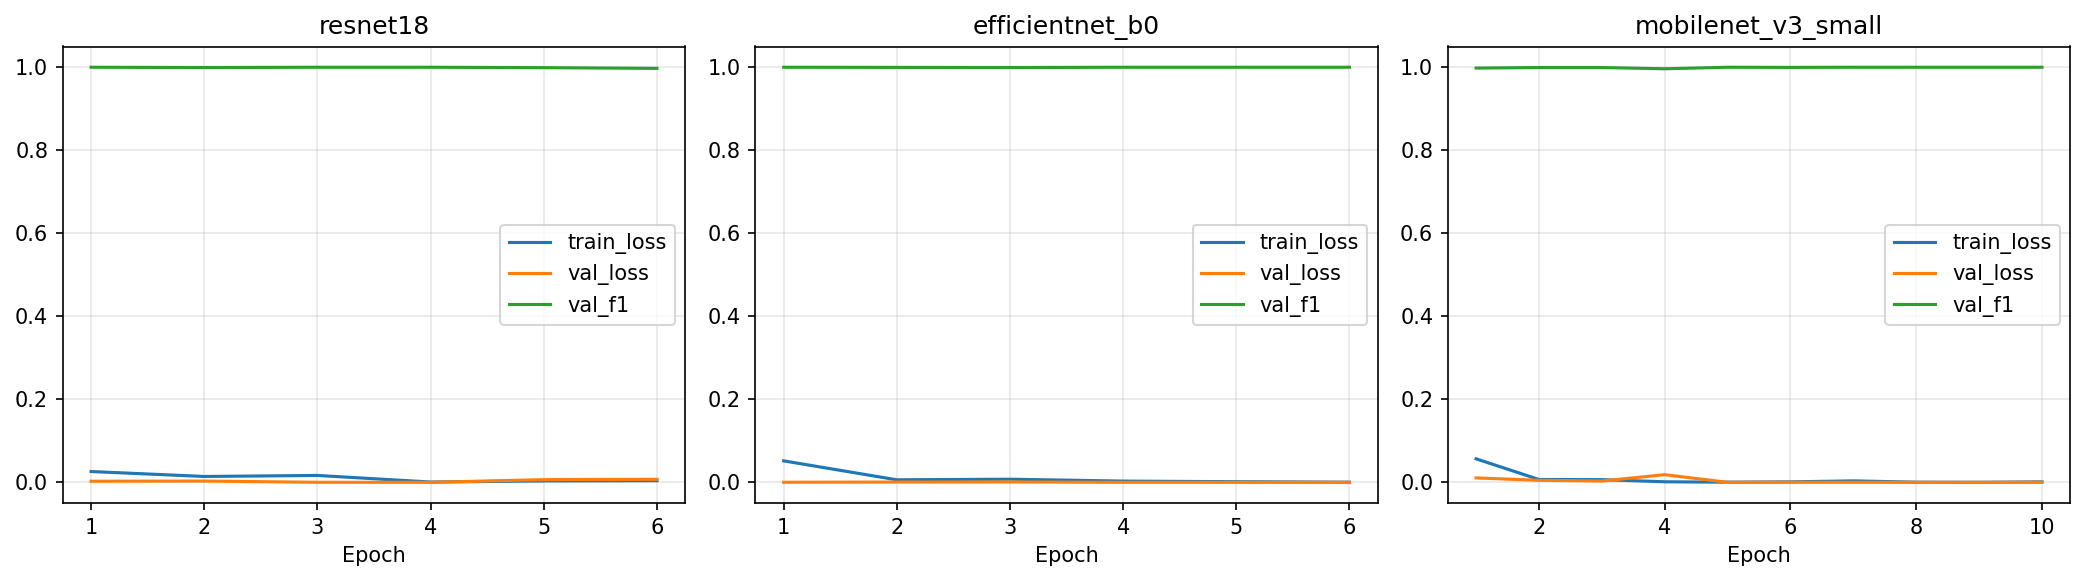
\includegraphics[width=0.98\textwidth]{figures/training_curves.png}
  \caption{Curvas de entrenamiento de los modelos preentrenados (pérdida train/val y
  evolución de F1): rápida convergencia sin sobreajuste aparente.}
  \label{fig:curvas-clf}
\end{figure}

\begin{figure}[H]
  \centering
  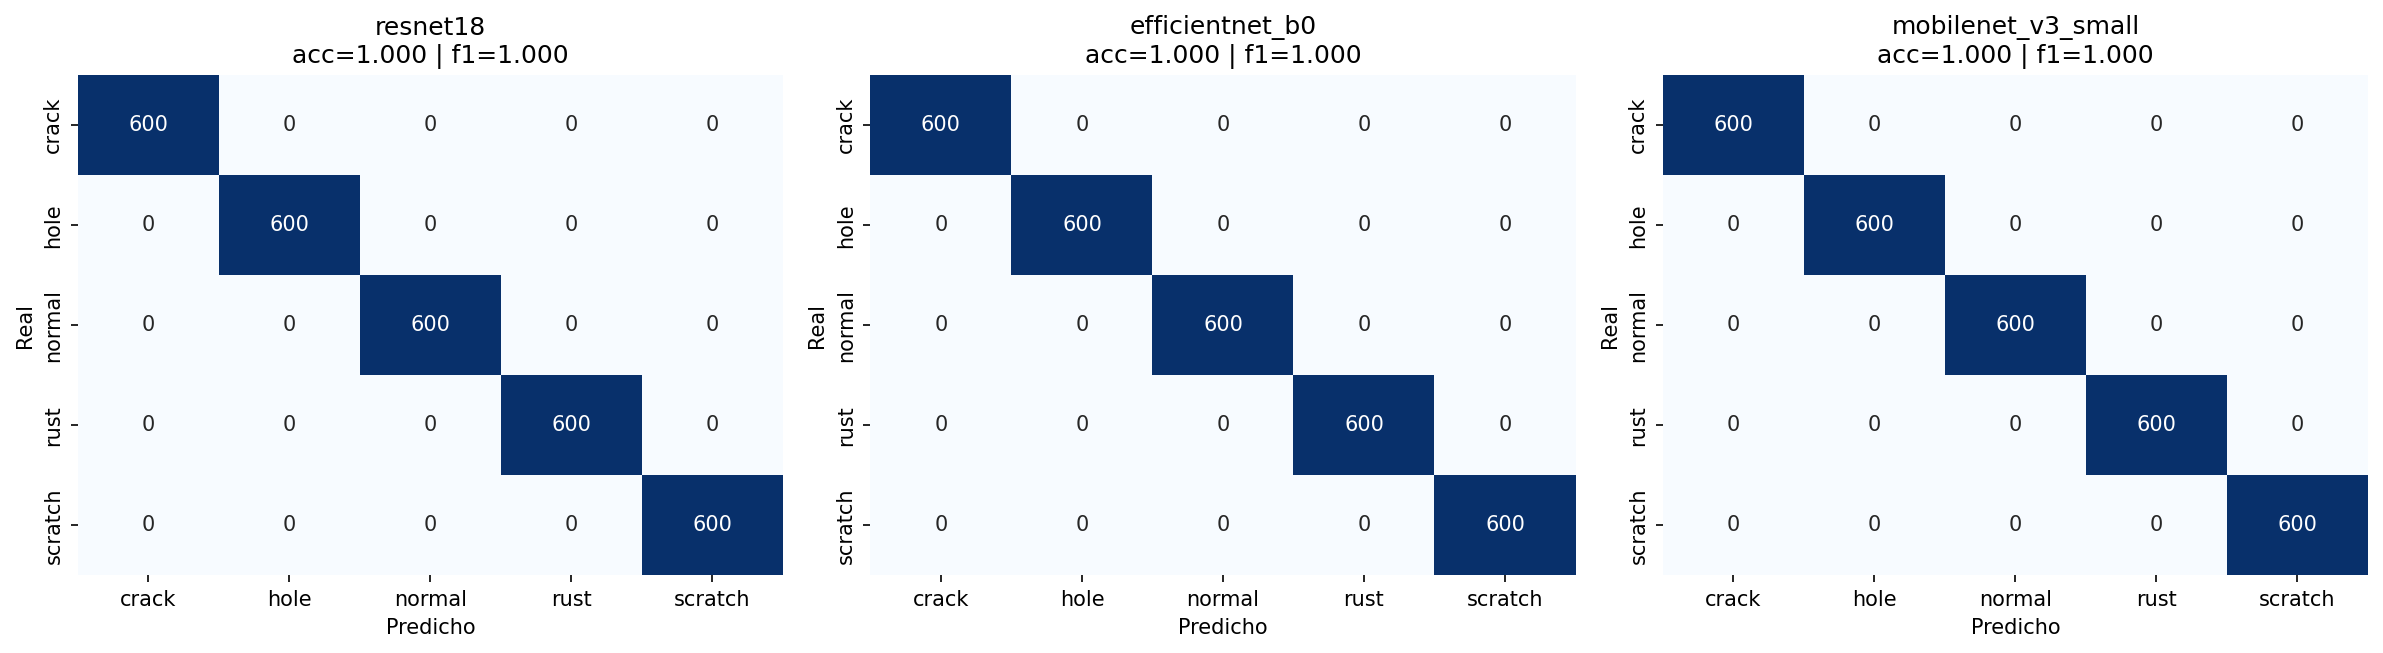
\includegraphics[width=0.98\textwidth]{figures/confusion_matrices.png}
  \caption{Matrices de confusión en test para los modelos preentrenados: diagonal pura
  (300 aciertos por clase en cada modelo).}
  \label{fig:cm}
\end{figure}

\begin{figure}[H]
  \centering
  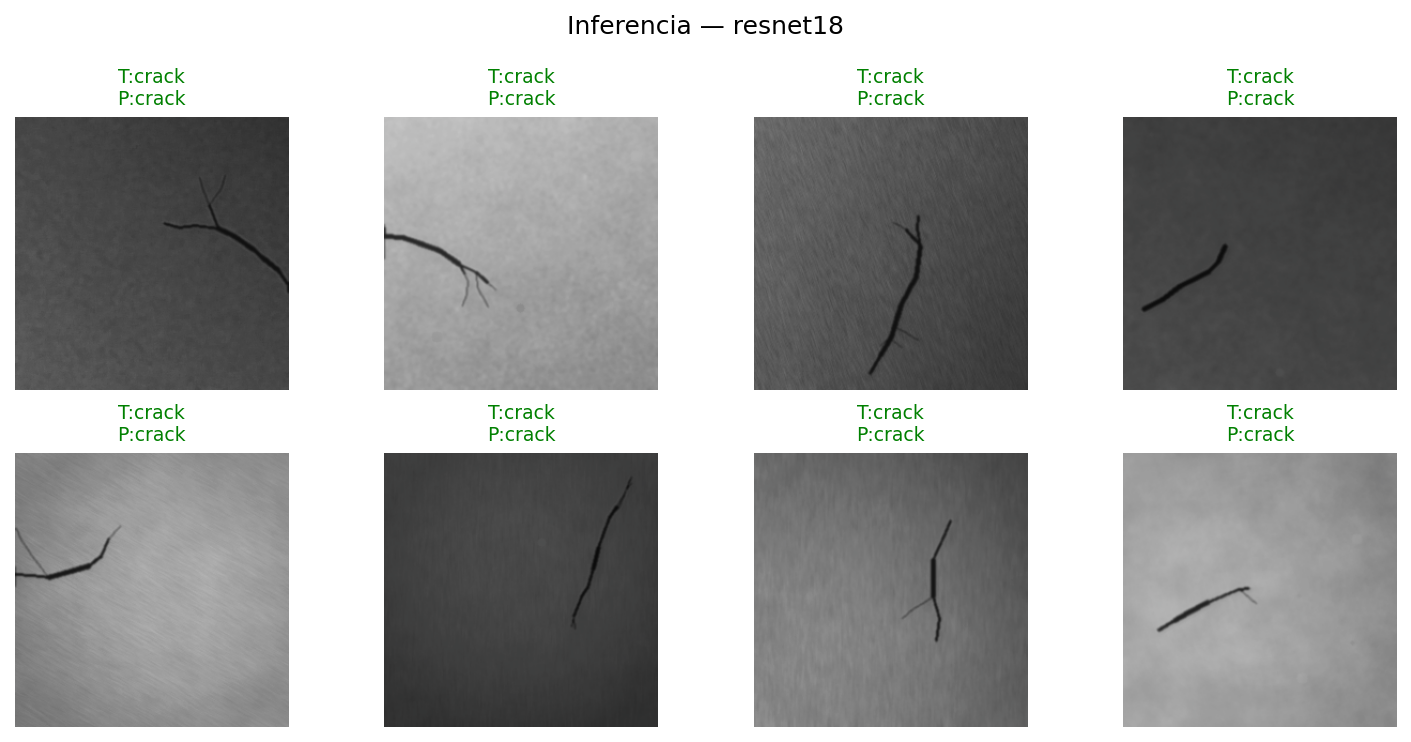
\includegraphics[width=0.88\textwidth]{figures/inference_predictions.png}
  \caption{Muestras de inferencia cualitativa en clasificación (ResNet-18) sobre imágenes de prueba.}
  \label{fig:infer}
\end{figure}

\subsection{Detección de objetos con YOLOv8n}
La evaluación del detector se ejecutó sobre el split de prueba combinado de 1\,725
imágenes (que integra 1\,500 sintéticas, 48 de SteelDefectX y 177 de NEU-DET con
cajas reales). En la Tabla~\ref{tab:det_global} y Tabla~\ref{tab:det_clase} se
desglosan las métricas cuantitativas obtenidas.

\begin{table}[H]
  \centering\small
  \caption{Métricas globales de detección de YOLOv8n sobre el conjunto de prueba (1\,725 imágenes).}
  \label{tab:det_global}
  \begin{tabularx}{\textwidth}{@{}l c c c X@{}}
    \toprule
    \textbf{Métrica} & $\text{\textbf{mAP}}_{50}$ & $\text{\textbf{mAP}}_{50\text{--}95}$ & \textbf{Precisión (\emph{Precision})} & \textbf{Exhaustividad (\emph{Recall})} \\
    \midrule
    \textbf{Valor} & \textbf{0.739} & \textbf{0.488} & \textbf{0.754} & \textbf{0.663} \\
    \bottomrule
  \end{tabularx}
\end{table}

\begin{table}[H]
  \centering\small
  \caption{Desempeño del detector YOLOv8n desglosado por clase de defecto.}
  \label{tab:det_clase}
  \begin{tabularx}{\textwidth}{@{}l c c X@{}}
    \toprule
    \textbf{Clase de Defecto} & $\text{\textbf{AP}}_{50}$ & $\text{\textbf{AP}}_{50\text{--}95}$ & \textbf{Comportamiento Físico Observado} \\
    \midrule
    \texttt{hole} (Perforación)  & \textbf{0.846} & \textbf{0.645} & Geometría delimitada, contraste nítido con el fondo. \\
    \texttt{crack} (Grieta)      & \textbf{0.791} & 0.541 & Alta precisión en fisuras continuas; sensible a aperturas finas. \\
    \texttt{rust} (Óxido)        & 0.677 & 0.407 & Bordes difusos y variabilidad de tonalidad superficial. \\
    \texttt{scratch} (Rayón)     & 0.643 & 0.361 & Trazos extremadamente finos sensibles a la resolución de $256\text{px}$. \\
    \midrule
    \textbf{Promedio Global (mAP)} & \textbf{0.739} & \textbf{0.488} & Rendimiento balanceado para inspección industrial. \\
    \bottomrule
  \end{tabularx}
\end{table}

\begin{figure}[H]
  \centering
  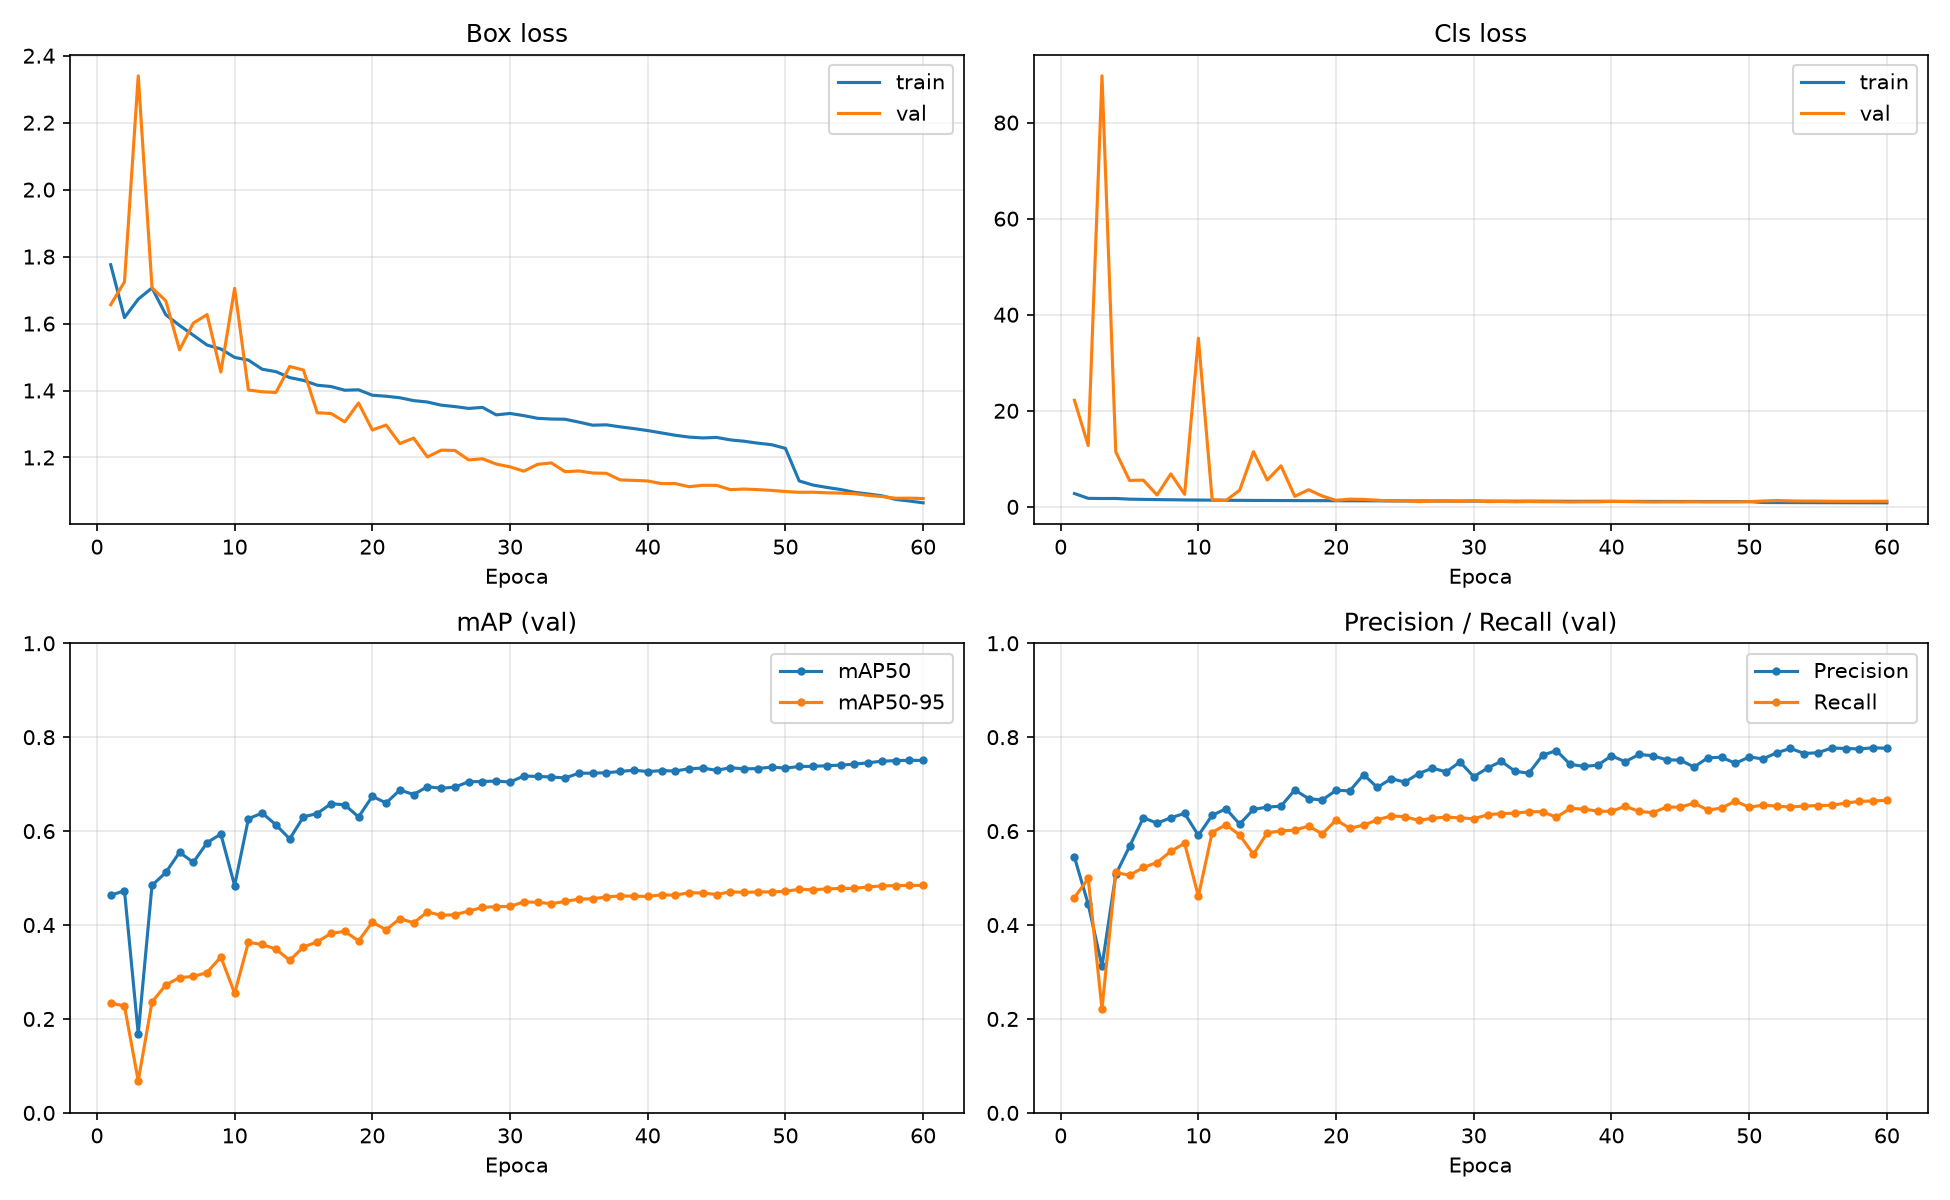
\includegraphics[width=0.98\textwidth]{figures/yolo_curvas.png}
  \caption{Curvas de aprendizaje de YOLOv8n durante 60 épocas de entrenamiento en GPU RTX 5060 Ti:
  pérdidas de caja y clasificación (train/val), y evolución de $\text{mAP}_{50}$, $\text{mAP}_{50\text{--}95}$,
  precisión y recall.}
  \label{fig:curvas-yolo}
\end{figure}

\begin{figure}[H]
  \centering
  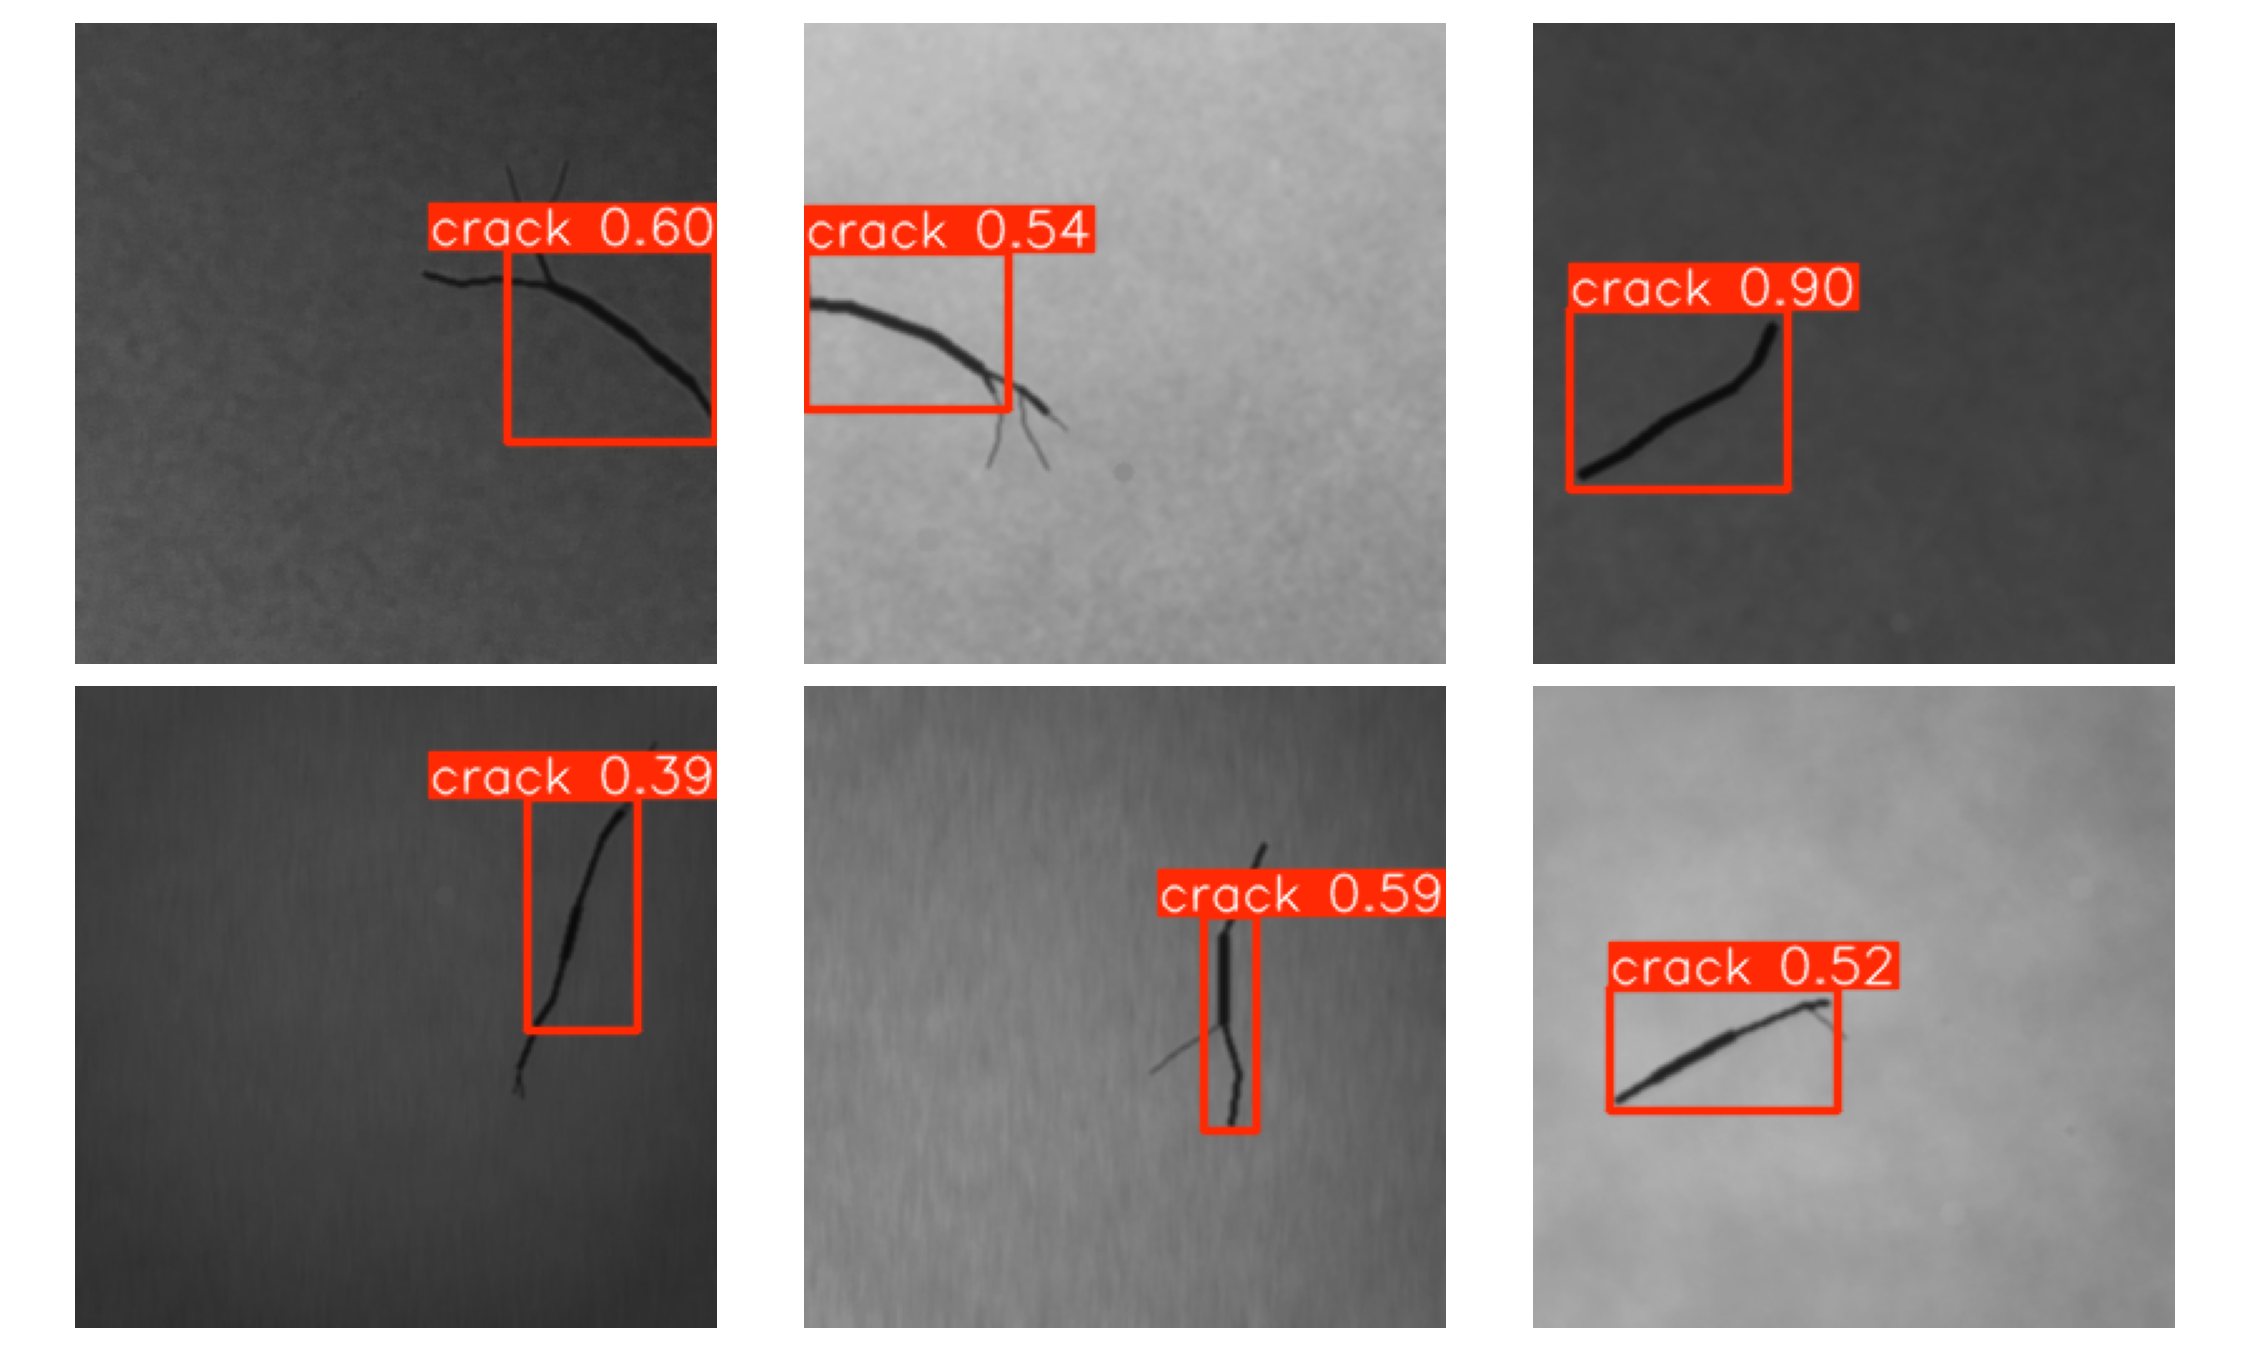
\includegraphics[width=0.92\textwidth]{figures/yolo_predicciones.png}
  \caption{Predicciones cualitativas de YOLOv8n sobre muestras de prueba: localización
  mediante caja delimitadora, asignación de clase y score de confianza.}
  \label{fig:pred-yolo}
\end{figure}

\subsection{Análisis cualitativo y diagnóstico de errores}
El análisis minucioso de las predicciones arrojó patrones sistemáticos sobre aciertos y
fallos (Fig.~\ref{fig:errores}):

\begin{itemize}[leftmargin=1.6em,itemsep=0.2em]
  \item \textbf{Caso A (Detección Correcta -- \texttt{hole}):} El detector localiza
  perforaciones circulares e inclusiones con alta precisión y puntuaciones de confianza
  superiores a 0.85, incluso en láminas con baja reflectancia o iluminación no uniforme.
  \item \textbf{Caso B (Falso Positivo -- \texttt{rust}):} Se observaron casos en
  donde texturas rugosas o bandas oscuras de rodillos industriales fueron clasificadas
  falsamente como óxido. \emph{Hipótesis:} La distribución de frecuencias espaciales y
  ruido de sensor en patrones difusos guarda una fuerte correlación visual con las
  texturas de óxido sintético.
  \item \textbf{Falsos Negativos en \texttt{crack} y \texttt{scratch}:} De los falsos
  negativos identificados con umbral de confianza $\ge 0.5$, la mayor proporción
  corresponde a fisuras y rayones muy tenues. Al reescalar las imágenes a $256\times256$,
  estas estructuras lineales ocupan apenas 1 a 2 píxeles de grosor, lo que dificulta
  el solapamiento estricto de intersección sobre unión (IoU) y reduce la puntuación de
  confianza del modelo.
  \item \textbf{Errores de Clasificación Baseline (2 fallos en 1\,500):} La CNN
  baseline confundió una grieta tenue con superficie \texttt{normal} (confianza 0.51 vs
  0.38) y un parche de óxido incipiente con \texttt{normal} (confianza 0.70), ambos en
  imágenes con contraste casi imperceptible.
\end{itemize}

\begin{figure}[H]
  \centering
  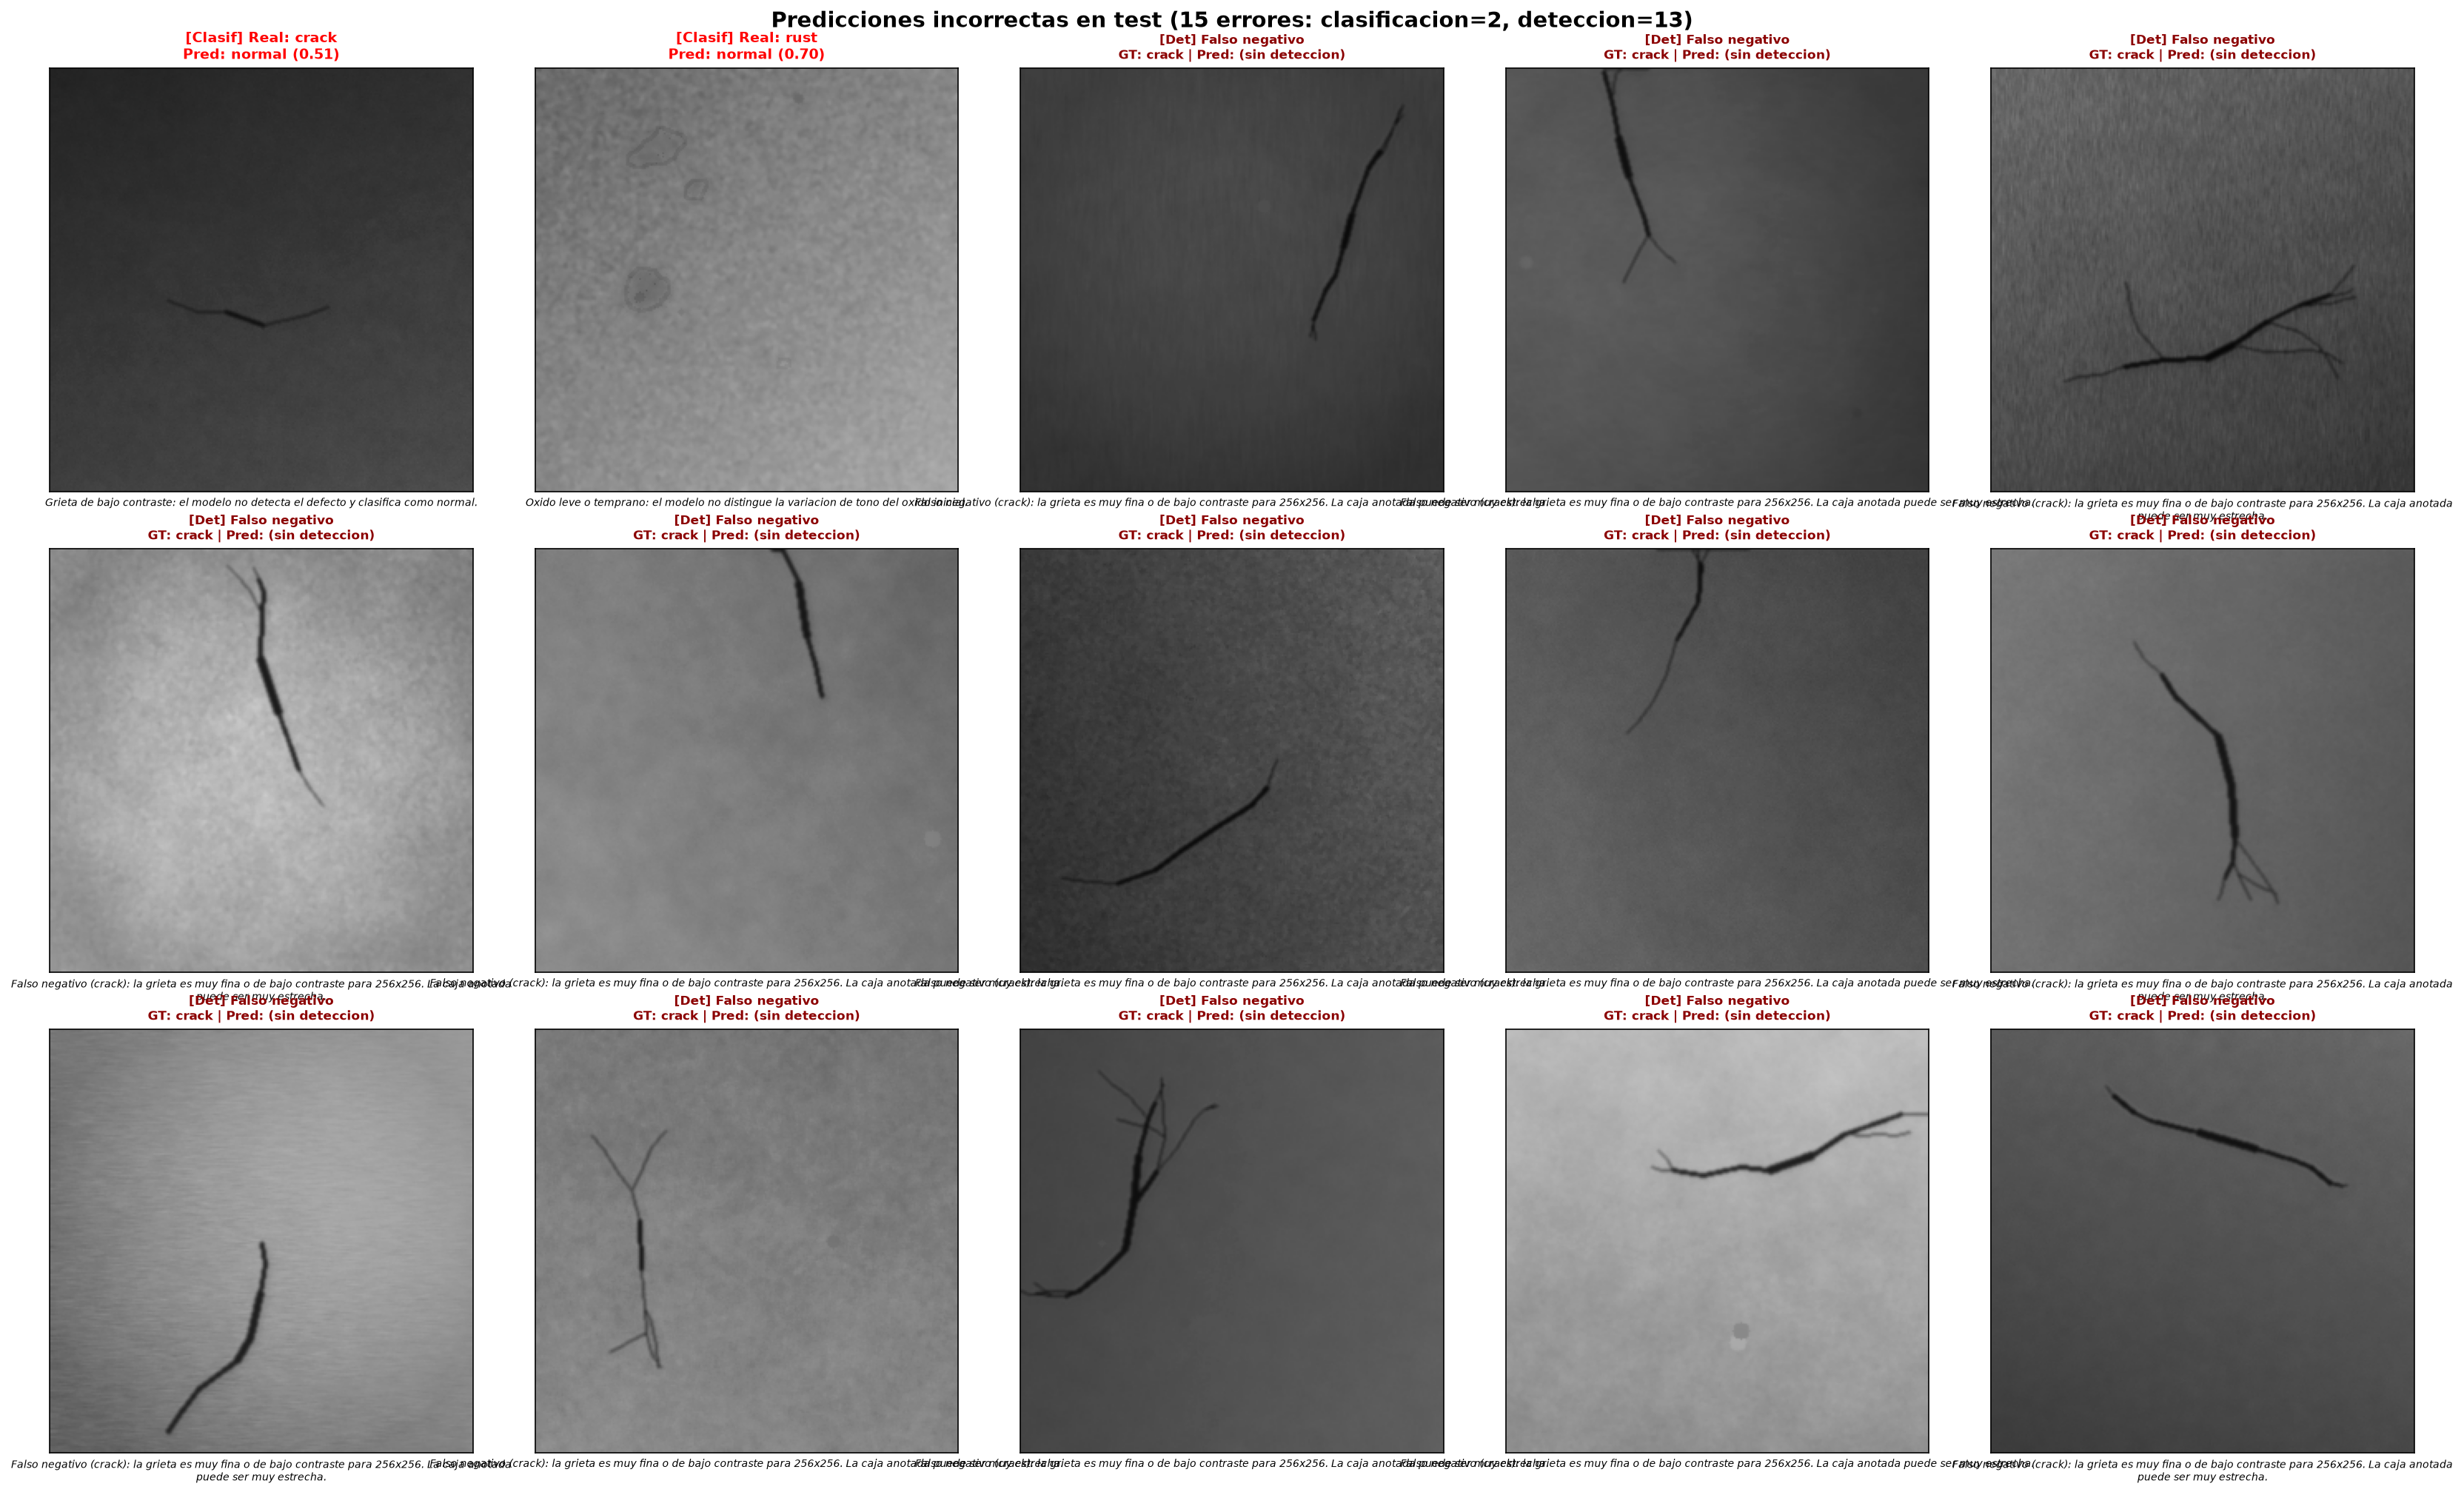
\includegraphics[width=0.98\textwidth]{figures/predicciones_incorrectas.png}
  \caption{Diagnóstico de predicciones erróneas en el conjunto de prueba. Fila superior:
  2 casos de clasificación incorrecta en la CNN baseline por bajo contraste. Filas
  inferiores: falsos negativos de YOLOv8n ($\text{conf} \ge 0.5$) en grietas y micro-defectos
  lineales a baja resolución.}
  \label{fig:errores}
\end{figure}

\subsection{Despliegue web e inferencia en tiempo real}
Ambos modelos fueron convertidos al estándar abierto ONNX (opset 17), validando la
paridad numérica exacta contra la ejecución en PyTorch (IoU medio de $1.0000$ en cajas
y concordancia en probabilidades de clase). 

El sistema cliente opera en navegadores web modernos mediante \textbf{ONNX Runtime Web}
y el backend de \textbf{WebAssembly (WASM) multi-hilo}, prescindiendo de servidores de
cómputo y garantizando la privacidad de los datos en planta. En pruebas de estrés se
alcanzaron tasas de \textbf{20--30+ FPS} en video en directo (Fig.~\ref{fig:demo}).

\begin{figure}[H]
  \centering
  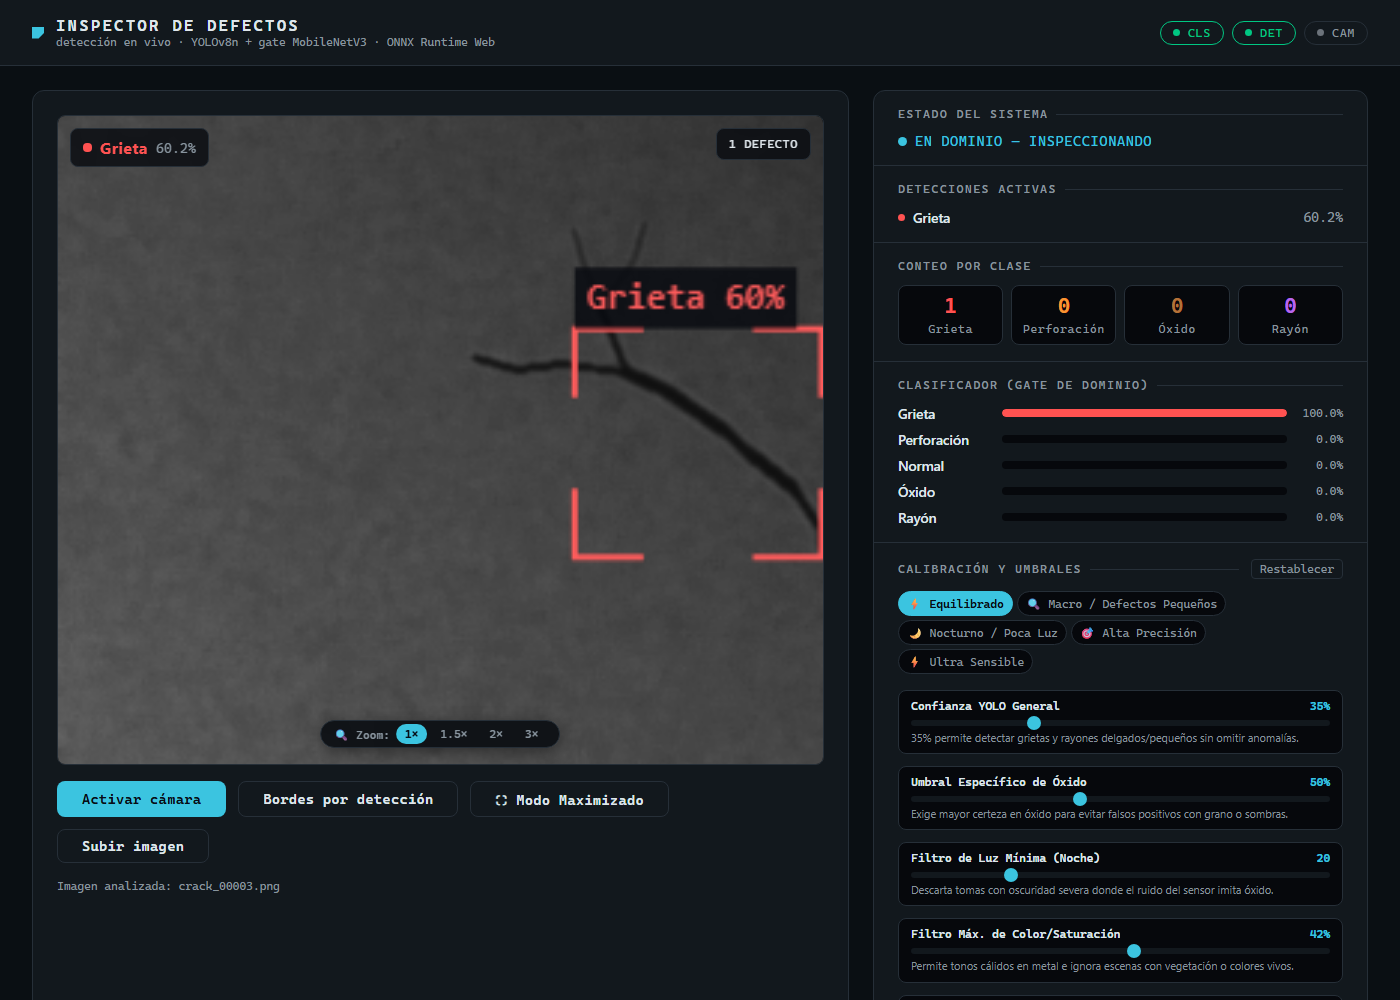
\includegraphics[width=0.48\textwidth]{figures/demo_crack.png}\hfill
  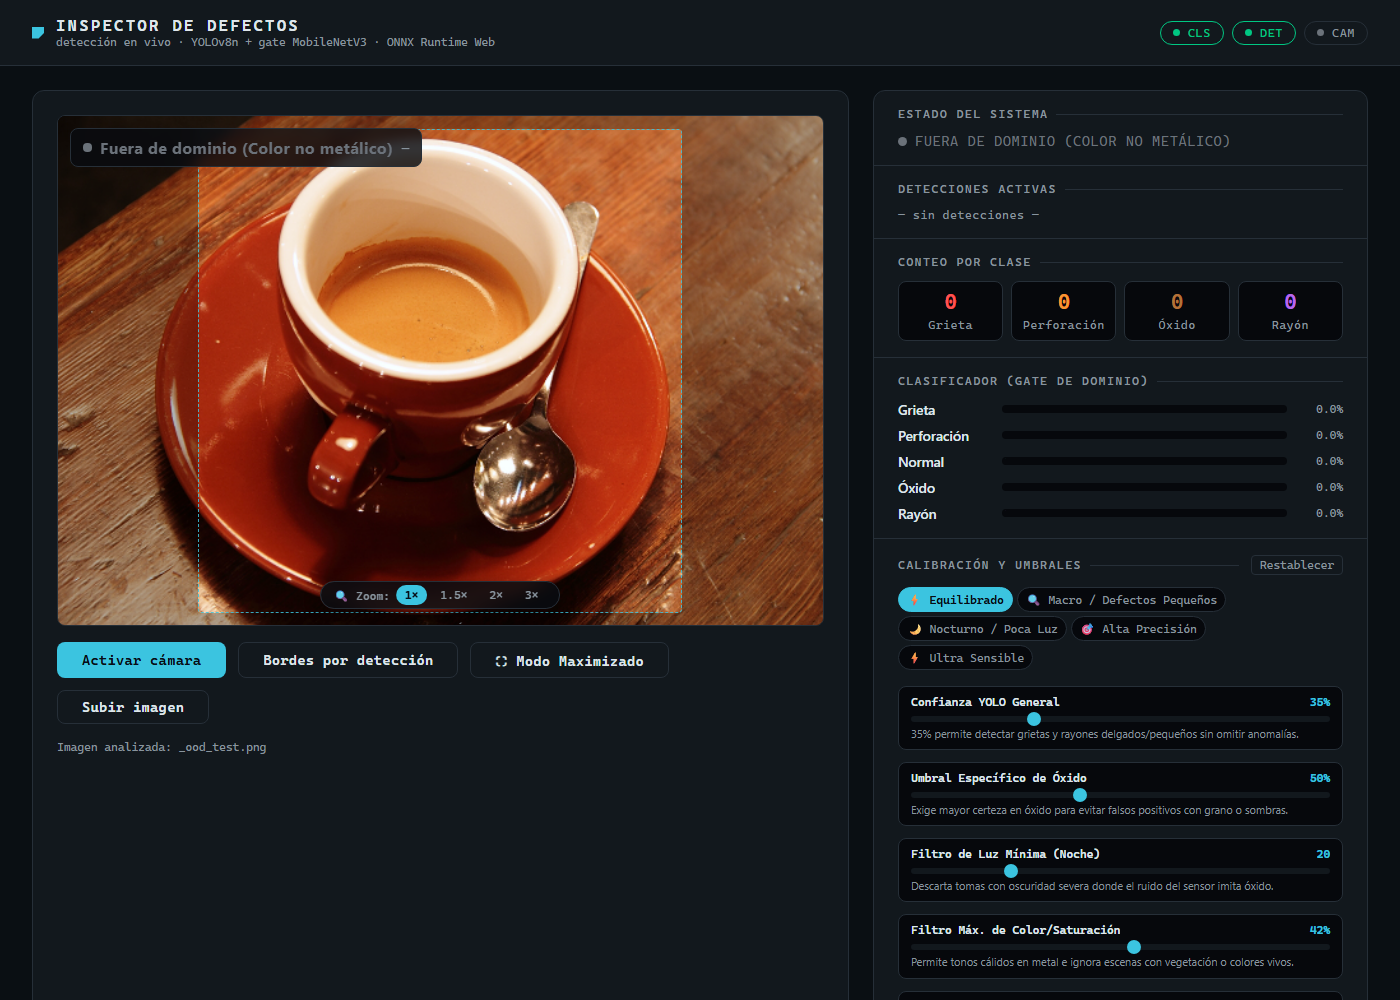
\includegraphics[width=0.48\textwidth]{figures/demo_ood.png}
  \caption{Validación operativa de la aplicación web en tiempo real. Izquierda: detección
  en vivo de grieta con caja y confianza. Derecha: el clasificador Gate rechaza una
  escena no industrial categorizándola como \emph{Fuera de Dominio} (OOD).}
  \label{fig:demo}
\end{figure}

% =================== 7. DISCUSIÓN Y LIMITACIONES ===================
\section{Discusión y limitaciones}

\textbf{Efecto de la inclusión de benchmarks reales:} Al integrar el dataset NEU-DET
en la evaluación, el $\text{mAP}_{50}$ global pasó de $0.80$ (en datasets exclusivamente
sintéticos o semi-heurísticos) a $0.739$. Lejos de considerarse un deterioro, este
resultado representa un avance metodológico positivo: NEU-DET incorpora anotaciones
manuales de expertos sobre piezas reales de acería, ofreciendo una métrica mucho más
honesta, rigurosa y cercana a las condiciones reales de planta.

\textbf{Validez de la clasificación perfecta (F1 = 1.0):} El resultado de F1-Macro
$=1.0000$ en los clasificadores con transfer learning debe interpretarse como una
\emph{cota superior en laboratorio}. Si bien el filtro Gate discrimina con absoluta
eficacia fondos no metálicos y escenas OOD sintéticas, la brecha \emph{sim-to-real}
sugiere que en planta la presencia de suciedad extrema, aceites de corte o cambios
bruscos de iluminación podría degradar ligeramente dicha métrica si no se recalibra
periódicamente.

\textbf{Ruido en etiquetas y regresión de cajas:} El uso de cajas heurísticas basadas
en segmentación por OpenCV para los datos sintéticos y SteelDefectX impone un techo a la
métrica $\text{mAP}_{50\text{--}95}$ ($0.488$). Una fracción de la pérdida de
localización (\emph{localization loss}) se debe a la imperfección geométrica de las
etiquetas de entrenamiento y no a una deficiencia intrínseca de la arquitectura de la red.

\textbf{Comportamiento de las curvas de entrenamiento:} Al completar las 60 épocas en
YOLOv8n, la curva de $\text{mAP}_{50}$ continuaba exhibiendo una pendiente positiva leve
sin saturación de \emph{early stopping}, lo que evidencia que un entrenamiento más
prolongado (100+ épocas) sobre el dataset consolidado de tres fuentes incrementaría aún
más la capacidad de detección.

% ========================= 8. TRABAJO FUTURO =========================
\section{Trabajo futuro}

A partir de los hallazgos del proyecto, se delinean tres líneas prioritarias de
extensión técnica:

\begin{enumerate}[leftmargin=1.6em,itemsep=0.2em]
  \item \textbf{Hardware de borde y cuantización INT8 (\emph{Edge Computing}):}
  Optimizar el grafo computacional mediante cuantización INT8 y TensorRT para su
  despliegue embebido en placas NVIDIA Jetson Orin / Xavier. Esto permitirá integrar
  la inferencia directamente en la óptica de las cámaras cenitales de la línea.
  \item \textbf{Refinamiento y curación manual de anotaciones:} Sustituir gradualmente
  las cajas generadas por algoritmos heurísticos de OpenCV por anotaciones 100\,\%
  validadas por inspectores de calidad humanos, cerrando la brecha de precisión
  geométrica en fallas lineales (\texttt{crack} y \texttt{scratch}).
  \item \textbf{Resiliencia ante ruido térmico y óptico:} Implementar bloques de
  preprocesamiento adaptativo y algoritmos de reducción de ruido (\emph{denoise}) para
  mitigar el ruido ISO elevado de los sensores y la distorsión por radiación infrarroja
  en entornos de laminación en caliente.
  \item \textbf{Aceleración WebGPU en el frontend:} Incorporar el backend de WebGPU en
  ONNX Runtime Web para triplicar la tasa de cuadros por segundo en equipos con GPU
  integradas o discretas sin consumo intensivo de CPU.
\end{enumerate}

% ========================== 9. CONCLUSIONES ==========================
\section{Conclusiones}

Este proyecto valida la viabilidad y efectividad de arquitecturas ligeras de aprendizaje
profundo (MobileNetV3-Small y YOLOv8n) para la inspección y aseguramiento de calidad en
la industria siderúrgica y metalúrgica en tiempo real. 

La arquitectura en cascada de dos etapas demuestra ser una estrategia de ingeniería
altamente robusta: el clasificador Gate asegura resiliencia ante entradas fuera de
dominio y fondos no pertinentes, mientras que el detector multiclase logra localizar y
discriminar defectos con un $\text{mAP}_{50}$ de $0.739$ sobre escenarios reales. 

La integración fluida del pipeline ---desde el entrenamiento acelerado en GPU hasta el
despliegue en navegador web a 20--30+ FPS mediante WebAssembly--- consolida una solución
práctica, escalable, privada y de bajo costo para la modernización de los procesos de
control de calidad industrial.

% ========================== 10. REFERENCIAS ==========================
\begin{thebibliography}{9}\small

\bibitem{neudet}
Song, K., \& Yan, Y. (2013).
\emph{A noise robust method based on completed local binary patterns for
hot-rolled steel strip surface defect detection}.
Applied Surface Science, 285, 858--864.
\url{https://doi.org/10.1016/j.apsusc.2013.09.002}

\bibitem{steeldefectx}
Zhao, X. et al. (2024).
\emph{SteelDefectX: A Real-World Benchmark Dataset for Steel Surface Defect
Detection}. Hugging Face Datasets.
\url{https://huggingface.co/datasets/Zhaosxian/SteelDefectX}

\bibitem{kaggle}
Abbas, T.
\emph{Synthetic Industrial Metal Surface Defects} (15\,000 imágenes, CC BY 4.0).
Kaggle Datasets.
\url{https://www.kaggle.com/datasets/tatheerabbas/synthetic-industrial-metal-surface-defects}

\bibitem{mobilenetv3}
Howard, A. et al. (2019).
\emph{Searching for MobileNetV3}.
IEEE/CVF International Conference on Computer Vision (ICCV), 1314--1324.

\bibitem{yolov8}
Jocher, G., Chaurasia, A., \& Qiu, J. (2023).
\emph{Ultralytics YOLOv8}.
\url{https://github.com/ultralytics/ultralytics}

\bibitem{resnet}
He, K., Zhang, X., Ren, S., \& Sun, J. (2016).
\emph{Deep Residual Learning for Image Recognition}.
IEEE Conference on Computer Vision and Pattern Recognition (CVPR), 770--778.

\bibitem{efficientnet}
Tan, M., \& Le, Q. (2019).
\emph{EfficientNet: Rethinking Model Scaling for Convolutional Neural Networks}.
International Conference on Machine Learning (ICML), 6105--6114.

\bibitem{onnxruntime}
Microsoft (2024).
\emph{ONNX Runtime Web: High performance machine learning inference in the browser}.
\url{https://onnxruntime.ai/}

\bibitem{datasheets}
Gebru, T. et al. (2018).
\emph{Datasheets for Datasets}.
arXiv:1803.09010.

\end{thebibliography}

\end{document}
